\documentclass[../main.tex]{subfiles}
\graphicspath{{\subfix{../images/}}}
\begin{document}
\section*{Term 1 Week 10}
\begin{enumerate}
    \item 
    Find the length of the radius of the circle:
    \begin{figure}[H]
        \centering
        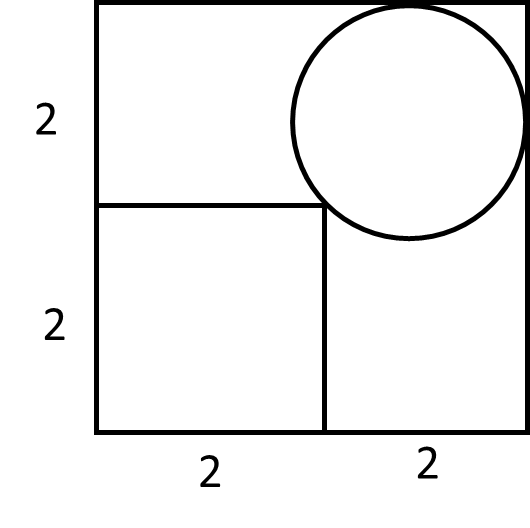
\includegraphics{images/t1w10q1.png}
    \end{figure}
    \item 
    Two vertical poles of respective heights 8m and 5m are standing on level ground. A rope is tied from the top of each pole to the bottom of the other.\\
    
    How high above the ground do the two ropes meet?
    \begin{figure}[H]
        \centering
        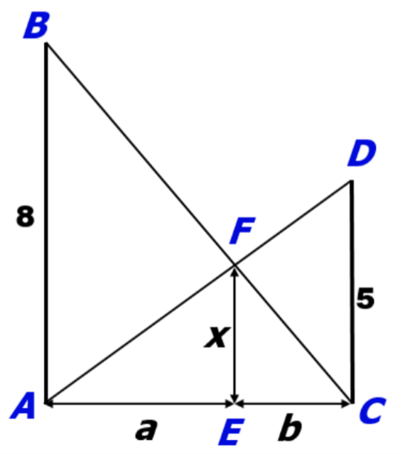
\includegraphics{images/t1w10q2.png}
    \end{figure}

    \item 
    Starting with a triangle, squares are constructed off each side. Three blue triangles are then created as shown in the diagram.\\
    
    What percentage of the original triangle is the total area of the three blue triangles?\\
    \begin{figure}[H]
        \centering
        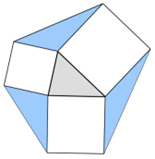
\includegraphics{images/t1w10q3.png}
    \end{figure}
    \item 
    A water tank is full of water. It has three outlet pipes, each having a constant drainage rate. Let a, b and c be labels for the outlet pipes.\\
    
    If a and b are both turned on, they take 12 hours to drain the tank.\\
    If a and c are both turned on, they take 15 hours to drain the tank.\\
    If b and c are both turned on, they take 20 hours to drain the tank.\\
    
    How long would each outlet pipe take to drain the water tank if they were opened individually?
    \begin{figure}[H]
        \centering
        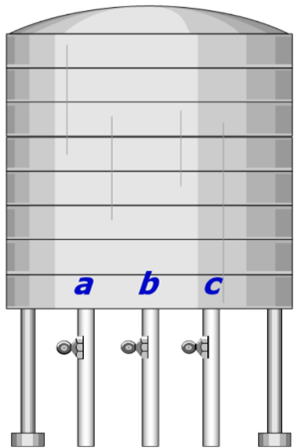
\includegraphics{images/t1w10q4.png}
    \end{figure}
\end{enumerate}

\end{document}